\title{A load-aware scheduler for large-scale neural network autotuning}
\author{Dominik Stiller}
\date{September 2019}

\documentclass{scrreprt}


%----------------------------------------------------------------------------
% Package Includes
%----------------------------------------------------------------------------
\usepackage[USenglish]{babel}
\usepackage[T1]{fontenc}
\usepackage[utf8]{inputenc}
\usepackage{lmodern}

\usepackage{tocloft}
\usepackage{chngcntr}
\usepackage{amsmath}
\usepackage{mathtools}
\usepackage{interval}
\usepackage{graphicx}
\usepackage[hidelinks]{hyperref}
\usepackage{geometry}
\usepackage{textcomp}
\usepackage{siunitx}
\usepackage{setspace}
\usepackage{array}
\usepackage[outputdir=build]{minted}
\usepackage{tabularx}
\usepackage{makecell}
\usepackage{csquotes}
\usepackage[toc,nonumberlist,acronym,nopostdot]{glossaries}
\usepackage[
	backend=biber,
	bibwarn=true,
	bibencoding=utf8,
	sortlocale=en_US,
	urldate=long,
	style=ieee
]{biblatex}
\usepackage[activate={true,nocompatibility},final,tracking=true,kerning=true,spacing=true,factor=1100,stretch=10,shrink=10]{microtype}


%----------------------------------------------------------------------------
% Package Config
%----------------------------------------------------------------------------

% KOMA-Script
\KOMAoptions{
	pagesize=pdftex,
	twoside=false,		% Einseitiger Druck.
	parskip=half,		% Halbe Zeile Abstand zwischen Absätzen.
	headheight = 12pt,	% Höhe der Kopfzeile
	headsepline,		% Linie nach Kopfzeile.
	footsepline,		% Linie vor Fusszeile.
	footheight = 16pt,	% Höhe der Fusszeile
	abstract=true,		% Abstract Überschriften
	DIV=calc,			% Satzspiegel berechnen
	%BCOR=8mm,			% Bindekorrektur links: 8mm
	headinclude=false,	% Kopfzeile nicht in den Satzspiegel einbeziehen
	footinclude=false,	% Fußzeile nicht in den Satzspiegel einbeziehen
	listof=totoc,		% Abbildungs-/ Tabellenverzeichnis im Inhaltsverzeichnis darstellen
	toc=bibliography	% Literaturverzeichnis im Inhaltsverzeichnis darstellen
}
\clubpenalty = 10000 % schließt Seitenumbruch nach der ersten Zeile eines neuen Absatzes aus
\widowpenalty = 10000 % schließt die letzte Zeile eines Absatzes steht auf einer neuen Seite aus
\displaywidowpenalty=10000

% graphicx
\graphicspath{ {./images/} }

% biblatex
\addbibresource{misc/references.bib}

% Microtype
% http://www.khirevich.com/latex/micrsotype/
\SetProtrusion{encoding={*},family={bch},series={*},size={6,7}}
			     {1={ ,750},2={ ,500},3={ ,500},4={ ,500},5={ ,500},
	             6={ ,500},7={ ,600},8={ ,500},9={ ,500},0={ ,500}}
\SetExtraKerning[unit=space]
   				{encoding={*}, family={bch}, series={*}, size={footnotesize,small,normalsize}}
				{\textendash={400,400}, % en-dash, add more space around it
	               "28={ ,150}, % left bracket, add space from right
	               "29={150, }, % right bracket, add space from left
					\textquotedblleft={ ,150}, % left quotation mark, space from right
					\textquotedblright={150, }} % right quotation mark, space from left
\SetExtraKerning[unit=space]
				{encoding={*}, family={qhv}, series={b}, size={large,Large}}
				{1={-200,-200}, \textendash={400,400}}
\SetTracking{encoding={*}, shape=sc}{40}
\microtypecontext{spacing=nonfrench}

% glossary
\renewcommand*{\glsgroupskip}{}

% chngcntr
\counterwithout{figure}{chapter}
\counterwithout{table}{chapter}
\counterwithout{equation}{chapter}

% minted
\usemintedstyle{friendly}
\newminted{python}{
	mathescape,
	linenos,
	numbersep=5pt,
	frame=lines,
	framesep=2mm
}
\newmintinline{python}{}

% amsmath
\DeclareMathOperator*{\argmax}{arg\,max}
% https://tex.stackexchange.com/a/43009
\DeclarePairedDelimiter\abs{\lvert}{\rvert}
\makeatletter
\let\oldabs\abs
\def\abs{\@ifstar{\oldabs}{\oldabs*}}
\makeatother


%----------------------------------------------------------------------------
% Styling
%----------------------------------------------------------------------------

% Page
\geometry{margin=2.5cm, foot=1cm}

% Font
\KOMAoptions{fontsize=12pt}
\DeclareMathSizes{12pt}{12pt}{15pt}{10pt}
\setkomafont{title}{\Huge\textbf}
\onehalfspacing

% Table of Contents
\setcounter{tocdepth}{1}


%----------------------------------------------------------------------------
% Custom Commands
%----------------------------------------------------------------------------

\newcommand*{\vcenteredhbox}[1]{
	\begingroup
	\setbox0=\hbox{#1}\parbox{\wd0}{\box0}
	\endgroup
}

\newcommand{\multilinecell}[2][c]{%
	\begin{tabular}
		[#1]{@{}l@{}}#2
	\end{tabular}
}


\makeglossaries
\newglossaryentry{machine learning}{
	name={ml},
	description={using computers}
}

\newacronym{cv}{CV}{computer vision}
\newacronym{ml}{ML}{machine learning}
\newacronym{ann}{ANN}{artificial neural network}
\newacronym{cnn}{CNN}{convolutional neural network}
\newacronym{gpu}{GPU}{graphics processing unit}

\begin{document}
	\pagenumbering{Roman}
	\pagestyle{empty}
	\makeatletter
	\begin{titlepage}
		\vcenteredhbox{
\includegraphics[height=2cm]{logo_hpe.png}}
\hfill
\vcenteredhbox{
\includegraphics[height=2cm]{logo_dhbw.png}}

\vfill
\begin{center}
	\rule{\textwidth}{1pt}
	{
		\Huge
		\bfseries
		A load-aware scheduler \\ for large-scale \\ neural network autotuning
		\par
	}
	\vspace{-0.2cm} 
	\rule{\textwidth}{1pt}

	\vfill

	\textsc{Project Thesis II / T2000}
	
	\vfill

	for the study program \\ \textbf{Computer Science}
	
	at the \\ \textbf{Baden-Wuerttemberg Cooperative State University Stuttgart}
	
	by \\ \textbf{\@author}
\end{center}

\vfill

\begin{tabbing}
	mmmmmmmmmmmmmmmmmmmmmmmmmm				\= \kill
	\textbf{Date}      						\> \@date \\
	\textbf{Project Period} 				\> 18 Weeks \\
	\textbf{Matriculation Number, Course}  	\> 4369179, TINF17A \\
	\textbf{Company}                        \> Hewlett Packard Enterprise \\
	\textbf{Corporate Supervisor}           \> Junguk Cho \\
	\textbf{University Supervisor}          \> Prof. Dr. Bernd Schwinn
\end{tabbing}

	\end{titlepage}
	
	\section*{Declaration of Authorship}
	I hereby declare that the thesis submitted with the title \textit{\@title} is my own unaided work. All direct or indirect sources used are acknowledged as references.

Neither this nor a similar work has been presented to an examination committee or published.

\vspace{4em}

Sindelfingen
\hspace{1.3cm}
September 12, 2019
\vspace{-0.4cm}
\\
\rule{15cm}{0.4pt}\\
Place
\hspace{2.5cm}
Date
\hspace{4.5cm}
\@author
	\makeatother

	\begin{abstract}
		Real-time computer vision applications with deep learning-based inference require hardware-specific optimization to meet stringent performance requirements. However, this approach requires vendor-specific libraries developed by experts for some particular hardware, limiting the set of supported devices and hindering innovation. The deep learning compiler stack TVM is developed to address these problems. TVM generates the optimal low-level implementation for a certain target device based on a high-level input model using machine learning in a process called autotuning.

In this paper, we first explore the capabilities and limitations of TVM's autotuning implementation. Then, we develop a scheduler to orchestrate multiple, parallel autotuning jobs on shared computation resources such as CPUs and GPUs, allowing us to minimize resource idle time and job interference. Finally, we reflect our design choices and compare the efficiency of our approach with the default, scheduler-less design.
	\end{abstract}

	\setlength{\cftbeforetoctitleskip}{0em}
	\begin{spacing}{1.15}
	   \tableofcontents
	\end{spacing}
	\clearpage
	\thispagestyle{empty}
	
	\pagestyle{plain}
	
	%----------------------------------------------------------------------------
	% Preface
	%----------------------------------------------------------------------------
	\printacronyms
	\clearpage
	
	\addcontentsline{toc}{chapter}{\listfigurename}
	\listoffigures
	\clearpage
	\addcontentsline{toc}{chapter}{\listtablename}
	\listoftables
	\renewcommand\listoflistingscaption{List of Source Codes}
	\listoflistings
	\clearpage
	
	\pagenumbering{arabic}
	
	\pagestyle{headings}
	
	\addtocontents{toc}{\protect\thispagestyle{empty}}
	\obeylines
	%----------------------------------------------------------------------------
	% Content
	%----------------------------------------------------------------------------
	\chapter{Introduction}
	In recent years, \gls{ai} has garnered tremendous success, revolutionizing the way we work and accelerating economic growth. It has the potential to increase growth rates of industries such as manufacturing and financial services by 2.1 and 1.9 percentage points respectively~\cite[p.~17]{Statista.2019}. Especially \gls{dl}, a subfield of \gls{ai}, has made vast improvements and is the prime method of modern \gls{ai}. In the future, \gls{ai} will be applied to even more areas, where non-expert users want to benefit from \gls{ai} without the technical complexity introduced by development and deployment of \gls{ai} applications. This is facilitated by platforms such as BlueData and Qubole, which automate infrastructure setup and provide user-friendly interfaces to make \gls{ai} and \gls{ai} more accessible. 

\section{Problem}
More and more applications like industrial monitoring or autonomous driving require real-time performance, most of them powered by \gls{dl}. Specialized accelerator hardware such as \glspl{gpu} or FPGAs are employed to speed up the computation-intensive inference. However, the model itself needs device-specific, low-level optimizations to harness the accelerator's full potential. Currently, these optimizations are manually developed by the device vendor who have deep knowledge of their hardware. \gls{dl} researchers, who want to experiment with new model types and high-level optimizations, are forced to wait until low-level implementations are supported by vendor libraries. Additionally, it causes vendor lock-in.

Automated performance optimization, called autotuning, creates low-level optimizations without the need for human experts in a vendor-agnostic way. This fosters innovation and helps meet increasing performance demands for a growing variety of models and accelerator devices. While autotuning is already employed, it has not yet reached widespread use, partially because it is still inconvenient to use. Offering autotuning as-a-Service can make it accessible for a larger audience to facilitate real-time \gls{dl} applications, but requires support for large-scale autotuning. However, inefficiencies in the autotuning process prohibit efficient scaling and, in turn, implementation of an Autotuning as a Service platform. To the best of our knowledge, there is no existing solution for scaling autotuning.

\section{Scope}
In this thesis, we design and create a prototypical implementation of a load-aware scheduler to enable large-scale autotuning. This scheduler controls multiple autotuning jobs that share computation resources to overcome the inefficiencies of current autotuning. We show that controlling the execution of multiple jobs by a load-aware scheduler makes large-scale autotuning more efficient in terms of
\begin{itemize}
	\item autotuning completion time,
	\item resulting inference performance, and
	\item hardware requirements.
\end{itemize}

First, we discuss manual and automated performance optimization before comparing two frameworks for autotuning (Chapter \ref{sec:background}). Next, we will develop a framework to examine capabilities and limitations of autotuning in different scenarios. This will allows us to find capabilities and limitations which we can leverage to scale autotuning (Chapter \ref{sec:using-tvm}). We will design and implement our scheduler which is used in our proposed reference architecture for Autotuning as a Service (Chapter \ref{sec:autotuning-scheduler}). Finally, we evaluate our scheduler design and show its benefits (Chapter \ref{sec:evaluation}). Our experiments show good results for resulting inference performance and hardware requirements.

No improvements are made to the autotuning process itself, but we base our work in the TVM~\cite{Chen.2018b} autotuning framework and enhance it with a further component. Also, we do not implement Autotuning as a Service. This thesis describes only a reference architecture, a prototype is described in~\cite{Cho.2019}.

This project was conducted by the \textit{Networking, IoT and Mobility Laboratory} of the \textit{Hewlett Packard Labs}.

	\chapter{Deep Learning}
	\section{Machine Learning}
\section{Neural Networks}
\section{Convolutional Neural Networks}
describe convolutions
	\chapter{Inference Optimization}
	The traditional machine learning workflow consists of training and inference.
The number of inferences heavily outweighs the number of trainings, since an unlimited number of inferences can be made once a model is trained, albeit model re-training is done periodically to improve accuracy.
Thus, the performance optimization of inference is an important field.
Reduction in inference time has advantages
- need less hardware to perform same number of inferences
- higher number of inferences with same hardware
- enables real-time applications such as autonomous driving or industrial monitoring
Especially in real-time applications, a lot of inferences are being made. every saved ms makes big difference
Look closer at Seagate

use of specific accelerator devices
Generic models perform poorly because they dont make full use of accelerator capabilities
Not only need capable accelerator, but also model that is attuned to leverage its full potential

\section{Tensor Operator Optimization}
additionally to traditional training and inference deep learning workflow, we introduce inference performance optimization to meet real-time requirements
include graphic showing train-inference vs train-optimize-inference

to optimize for minimal inference time of whole network, we need to optimize implementation of every layer, or rather the respective tensor operator with the specific parameters (shape, padding, stride) in the computation graph
especially conv2d, because there are many and they are very computationally intensive
Dense not so important because less computational intensive (number?)

WHAT should be calculated is determined by model
HOW it should be calculated is not specified, so actual implementation can change
simple default implementation, but also loop unrolling, tiling, threads, example code?

It is important to note that the optimal implementation (regarding speed, memory usage) is very much dependent on target device
memory sharing and data reuse

\section{Manual Optimization}
state of the art cuDNN and TensorRT and Intel MKL, taken as baseline
requires deep knowledge of target device, usually provided by vendor
limitations
- no support for new devices
- no support for unconventional shapes
- no support for new graph-level optimizations
elaborate limitations
high-level optimization need to wait until vendor provides low-level support


\section{Automated Optimization}
vendor-agnostic and does not require expert knowledge
Enables innovation by enabling high-level optimization and fostering experimentation with unconventional layers, not supported by manual frameworks
describe autotuning process on high level
definition of search space (loop unrolling, tiling, threads)
Problem: search space is very large (billions), and any one of them could be the best one for one target device

impossible to try all
autotuning frameworks have some solution to explore search space rapidly
look at TVM and TC

has same or even better performance than hand-optimized libraries
show numbers

There are two frameworks that implement autotuning

\subsection{TensorComprehensions}
does not use machine learning

\subsection{TVM}
using machine learning
TVM is framework that proposed and implements autotuning

import from many frontends, compilation for many backends
has own graph-level and tensor operator-level representation
calls target-specific compiler

define autotuning job, task
first extraction of tasks
schedules as abstraction with knobs
details of autotuning process
Profiling repeated multiple times
RPC allows autotuning logic to run on powerful server, but profiling to happen on target device
with figure

In this project, we use TVM because of the novel, machine learning-based approach
Using (commit id) with a few modifications to support measurements (check what else we changed)

	\chapter{SimpleTVM}
	Using TVM follows the same workflow every time
To be able to quickly test different scenarios, we created a simpler interface for TVM, called SimpleTVM

\section{Design}
created wrapper for simpler usage of TVM
expose easy, chainable interface
Created automated benchmarking framework superb
enable automated testing of different configurations to be able to run multiple configurations without human intervention

Docker container to be able to easily deploy TVM with all dependencies on any server

\section{Exploration}
Using SimpleTVM and superb, it was easy to explore TVM behavior in different configurations of concurrency and resource sharing
First phase of experiments to investigate impact of interference
Evaluation in Jupyter notebooks

\section{Autotuning Limitations}

\subsection{Resource Utilization}
We noticed lots of resource idle time due to synchronous design
Show figure from poster
Want to minimize idle time because edge resources are limited (define edge)
Fundamental restriction due to dependencies of stages, cannot be changed for a single job

\subsection{Scalability}
Our goal is to enable large-scale autotuning for our AaaS, autotune multiple models at the same time

objectives:
Be able to run an arbitrary number of autotuning jobs while
1. maximizing inference performance: ultimate goal of autotuning
2. minimize hardware requirements: save cost
3. minimizing autotuning time: make autotuning worth the effort
in order of priority
State that autotuning time is not as crucial since it is rendered negligible by a large amount of inferences

With default tvm, there are two possible setups
Include figure with two setups
Include table with three experiments here

1. two completely separate autotuning jobs running independently on additional dedicated servers, one autotuning runner per server
Pros: good autotuning and inference time
Cons: Costly because we need multiple sets of the same hardware
not an economically feasible approach. We cannot simply use machines from a PaaS provider since actual target device needs to be used
Alternatively, we could use the same server and run them in sequence, trading off hardware required for autotuning time

2. two autotuning runners sharing the same server
Pros: only one set of hardware
Cons:
- interference drives up autotuning time
Autotuning takes long (in our tests anywhere between 3 and 36 hours, depending on hardware and network size)
Especially update model takes 64\% longer when two jobs are running simultaneously
- results in worse inference performance because profiling is distorted (show numbers)

In both setups, we do not meet all objectives
Gets worse the more jobs we add
AaaS is not possible efficiently with current implementation and architecture of autotuning in TVM, does not scale well

Ideally:
Prevent interference, because it affects autotuning time and inference performance
Minimize hardware required by utilizing available hardware fully before adding new servers for cost reasons

However, there does not seem to be any solution yet

\subsection{Similar Problems}
In general, problem can be formulated as follows:
How can resources be shared optimally between multiple tasks that are partially idle?

Add two examples
	\chapter{Autotuning Scheduler}
	Interleaving of the stages of multiple jobs is our key concept for enabling large-scale autotuning. \cite{Ma.2005} uses a design-time scheduler to create a program with good concurrency. We need to dynamically schedule incoming jobs, so the schedule cannot be predetermined. We need an additional component in the autotuning architecture that orchestrates running jobs. In this chapter, we describe the design and implementation of our central scheduler that controls stage execution.

\section{Design}
Our scheduler possesses the two features that have been determined to be imperative for optimal large-scale autotuning:
\begin{itemize}
	\item Computation resources are shared between jobs. This facilitates good resource utilization since the idle time of one job can be harnessed to execute another job. This is called \textit{interleaving} and saves hardware and costs as a result. However, stage dependencies of a single job must be maintained.
	\item Interference between jobs is prevented. This guarantees that inference performance and autotuning time are as good as possible. The scheduler needs to check if the resource that will be used by the next stage is free before execution. This might necessitate the postponing of stage executions if the stage is ready before the resource becomes free.
\end{itemize}
These two features not only make it match the optimal solution, but also do they solve the problem of bad resource utilization of single-job autotuning by leveraging that shortcoming.

\begin{figure}[h]
	\centering
	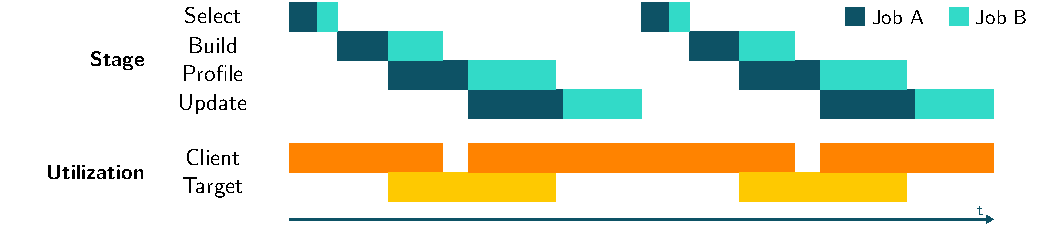
\includegraphics[width=\textwidth]{tvm_resource_utilization_interleaving}%
	\caption{Interleaving of multiple autotuning jobs}
	\label{fig:interleaving}
\end{figure}

Figure \ref{fig:interleaving} illustrates round-robin-based interleaving with an example of two jobs. Significant events are marked with numbers. Job A and Job B are started at the same time, but assume that the scheduler knows about A earlier. The first stage of A is executed, then the first stage of B. Once B finishes, the scheduler decides it is A's turn again and executes its second stage. Once A finishes the seconds stage, the client machine is free and B can execute the second stage. At the same time, A is ready to execute the third stage which will run on the target device. Since the target device is not in use, A can execute the profiling there in parallel to B's building since they use separate resources (\textbf{\textit{1}}). Building does not take as long as profiling, so A is ready to profile before B finishes its profiling stage. Therefore, A's third stage is postponed until the target device is free (\textbf{\textit{2}}). A's profiling and B's update model can, once again, execute simultaneously since they use distinct resources. After one iteration of all four stages, the process starts anew with the first stage (\textbf{\textit{3}}). This continues until both jobs are done. In a real scenario, new jobs might appear while other jobs are already running. The scheduler simply adds them to its list of jobs and includes them in the interleaving. Note how the resource utilization in Figure \ref{fig:interleaving} is much improved over the single-job autotuning in Figure \ref{fig:tvm-res-util} due to overlapping and sharing. Especially on the client device, utilization has almost been maximized since three of the four stages use the client.

\subsection{Autotuning Decomposition}
The default autotuning process is monolithic and can be regarded as a blackbox from the outside (Figure \ref{fig:autotuning-decomposition-before}). This means, the autotuning loop can be started, and it does not finish until the whole job is completed. Once a stage finishes, the next one is executed immediately. However, the scheduler needs to be able to control the execution of the individual stages because it needs to prevent interference by means of delayed execution. This necessitates the decomposition of the autotuning process into schedulable units, corresponding to the stages  (Figure \ref{fig:autotuning-decomposition-after}). The client does not execute any of the stages on its own. Rather, it provides an interface to execute schedulable units and waits for an external trigger to do so. The autotuning loop can now run in another component, such as the scheduler.

\begin{figure}
	\begin{minipage}[b]{.5\textwidth}
		\centering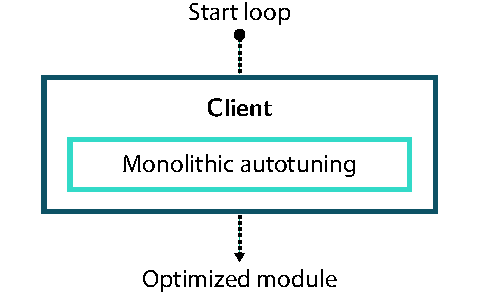
\includegraphics{autotuning_decomposition_before}
		\subcaption{Before decomposition}\label{fig:autotuning-decomposition-before}
	\end{minipage}%
	\begin{minipage}[b]{.5\textwidth}
		\centering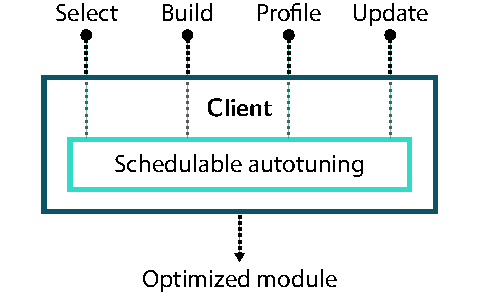
\includegraphics{autotuning_decomposition_after}
		\subcaption{After decomposition}\label{fig:autotuning-decomposition-after}
	\end{minipage}
	\caption{Client interface before and after decomposition}
	\label{fig:autotuning-decomposition}
\end{figure}

\subsection{Scheduling Algorithm}
To fulfill the task of interleaving while preventing interference, the scheduler needs to know four pieces of information for every job:
\begin{itemize}
	\item Whether the current stage is done; lets scheduler know if the job is ready for next stage
	\item Whether the whole job is done; lets scheduler know if the job needs to be considered in the future
	\item Which resource the current stage runs on; lets scheduler know which resources are free and which are in use
	\item Which resource the next stage will run on; lets scheduler postpone stage execution to prevent interference
\end{itemize}
We call this \textit{load-awareness}; being aware of the state of jobs and resources as well as their relationships. Theoretically, this allows the scheduler to work not only with TVM's autotuning but any process that can provide this information. Designing our scheduler to be agnostic of the underlying process also simplifies the algorithm since no state of this process, i.e. the progress or position in the loop, needs to be considered.

In case multiple jobs are ready to execute a stage, the scheduler needs to decide which one to run. The simplest approach is to use a round-robin algorithm, which iterates over the jobs in the order they were started and picks the first one that is ready. More sophisticated approaches might apply some logic to decide on a job which would maximize resource utilization but keep the average autotuning time low. However, we choose the round-robin algorithm for our first version. It is easy to implement and works reasonably well for an arbitrary number of jobs, which allows us to proof our concept.

We present two algorithms that perform interleaving. The greedy algorithm lets a job execute the next stage directly after the previous one finishes, provided the resource is free. This might preempt the resource from another job who is already waiting to execute a stage on it. On the other hand, the fair scheduler features a queue for every resource, so the first job to be ready to run a stage on a resource will be the first one to actually use it. Each job is controlled using an interface that provides the four pieces of information necessary for scheduling (\pythoninline/is_stage_done()/, \pythoninline/is_complete()/, \pythoninline/previous_resource/, \pythoninline/next_resource/). The scheduler keeps a list of jobs (\pythoninline/jobs/) in the order in which they were registered. With each call of \texttt{next()}, the subsequent job is returned, wrapping around after the end is reached.  Furthermore, it keeps a list of resources which can be marked as free or busy (\pythoninline/mark_as_free()/, \pythoninline/mark_as_busy()/).
\begin{description}
	\item[Greedy interleaving] The algorithm for greedy interleaved scheduling is presented in Listing \ref{lst:sched-algo-interleaving-greedy}. The algorithm is an infinite loop, with each iteration operating on one job (Line 1). First, the next job in the job list is retrieved (Line 2). If there is no job, the algorithm tries again until one is registered (Lines 3--4). If the job is still busy executing a stage, it is not considered further in this iteration (Line 6). If the stage has finished, the resource it used is marked as free (Line 7). If the stage was the last stage in the job, the job can be removed from the list of jobs (Line 8--9). Otherwise, the job is ready to continue. If the next stage's resource is free, that resource is marked as busy and the stage is executed immediately (Lines 11-13).
\begin{listing}[h]
\begin{pythoncode}
while True:
    job = jobs.next()
    if not job:
        continue

    if job.is_stage_done():
        mark_as_free(job.previous_resource)
        if job.is_complete():
            jobs.remove(job)
            continue
        if is_free(job.next_resource):
           mark_as_busy(job.next_resource)
           job.next_stage.execute()
\end{pythoncode}
\unskip
\caption{Greedy interleaved scheduling pseudocode}
\label{lst:sched-algo-interleaving-greedy}
\end{listing}
	\item[Fair interleaving] The algorithm for fair interleaved scheduling is presented in Listing \ref{lst:sched-algo-interleaving-fair}. Each resource has a queue which contains stages that are ready and will use that resource (Line 1). The algorithm is an infinite loop (Line 2), with each iteration consisting of two phases: scheduling and execution. In the first phase, the scheduler checks for each job if the current stage is done (Lines 4--5). Busy jobs are not regarded further. If the stage is done, the resource that was used is marked as free (Line 6). If the job is complete, it can be removed from the list of jobs (Line 7--8). Otherwise, the job is ready to continue and the next stage is added to the queue of the resource that it will run on (Line 9--10). The iteration over all jobs in order is what effectively makes this round-robin scheduling. In the second phase, the scheduler iterates over each resource and the corresponding queue (Line 12). If the resource is free and there are pending stages for that resource, the first stage in the queue is dequeued and executed (Lines 13--15). The respective resource needs to be marked as busy (Line 16).
\begin{listing}[h]
\begin{pythoncode}
queues = {r: [] for r in resources}
while True:
 # Phase 1: Round-robin scheduling
 for job in jobs:
     if job.is_stage_done():
         mark_as_free(job.previous_resource)
         if job.is_complete():
             jobs.remove(job)
         elif not job.next_stage in queues[job.next_resource]:
             queues[job.next_resource].enqueue(job.next_stage)
 # Phase 2: Execution
 for resource, queue in queues:
     if is_free(resource) and len(queue) > 0:
         stage = queue.dequeue()
         stage.execute()
         mark_as_busy(resource)
\end{pythoncode}
\unskip
\caption{Fair interleaved scheduling pseudocode}
\label{lst:sched-algo-interleaving-fair}
\end{listing}
\end{description}

Additionally to interleaving, our scheduler supports two other strategies for executing multiple jobs, which will be used in the evaluation for comparison.

Sequential scheduling (Listing \ref{lst:sched-algo-sequential}) works similar to single-job autotuning without a scheduler. Jobs do not run in parallel, but the next job is only started when the previous one finishes. This renders consideration of resource free/busy state unnecessary, and stages do not need to be postponed. However, since it is controlled by the scheduler, we can calculate the overhead introduced by adding a scheduler component, e.g., due to communication between scheduler and client or scheduling itself.

\begin{listing}[t]
\begin{pythoncode}
while True:
    job = jobs.next()
    if not job:
        continue

    while not job.is_complete():
        if job.is_stage_done():
            job.next_stage.execute()
    jobs.remove(job)
\end{pythoncode}
\unskip
\caption{Sequential scheduling pseudocode}
\label{lst:sched-algo-sequential}
\end{listing}

Synchronous scheduling (Listing \ref{lst:sched-algo-synchronous}) forces parallel execution of the same stage of multiple jobs on the same resource, making it the exact opposite of interleaved scheduling. Postponed stage execution is applied here to guarantee full interference. We use this strategy to evaluate the worst case effect of interference. However, this only works for equal jobs, since there needs to be symmetry between stages of all jobs.

\begin{listing}[t]
\begin{pythoncode}
while True:
    current_jobs = jobs
    if len(current_jobs) < 2:
        continue

    while not any([j.is_complete() for j in current_jobs]):
        if all([j.is_stage_done() for j in current_jobs]):
            [j.next_stage.execute() for j in current_jobs]
    jobs.remove_all(current_jobs)
\end{pythoncode}
\unskip
\caption{Synchronous scheduling pseudocode}
\label{lst:sched-algo-synchronous}
\end{listing}

\subsection{Autotuning Process}
\begin{figure}[ht]
	\centering
	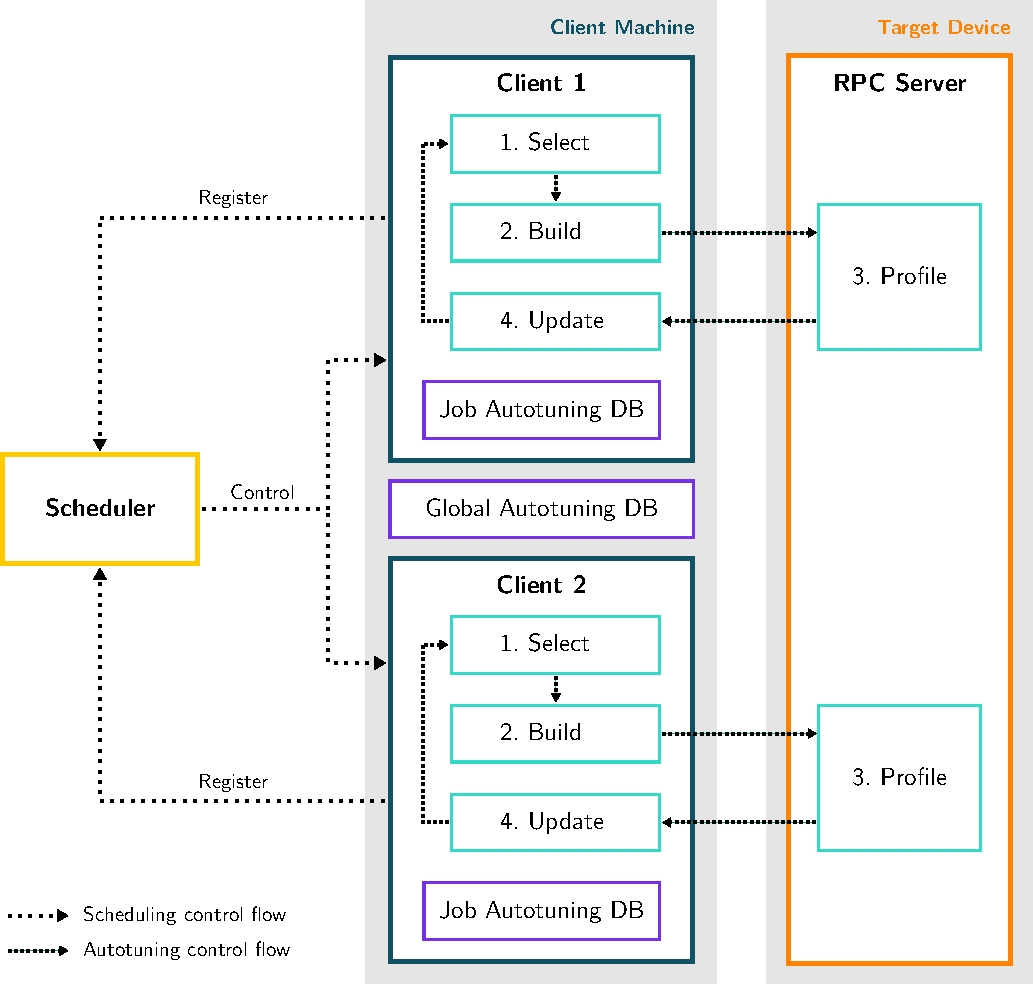
\includegraphics[width=\textwidth]{tvm_autotuning_with_scheduler.pdf}%
	\caption{Autotuning process with scheduler}
	\label{fig:tvm-autotuning-with-scheduler}
\end{figure}

Figure \ref{fig:tvm-autotuning-with-scheduler} shows the autotuning process with our scheduler (compare with scheduler-less, single-job autotuning in Figure \ref{fig:tvm-autotuning}). There are two discrete control flows at work. The per-job autotuning control flow is the same as before, spanning client and target machines. The scheduling control flow is on a higher level incorporating multiple jobs, and spans scheduler and clients. A new job needs to be made known to the scheduler first so it can consider the job in scheduling. One client is responsible for running exactly one job, registering that job with the scheduler when launching. The client is then ready to receive control commands to execute individual stages. The client exposes the interface which is required by the scheduling algorithm while calling the respective TVM methods internally. Clients can share target devices since the scheduler prevents interference of the profiling stages of multiple jobs on the same resource. The normal autotuning process is then executed, however not in one monolithic step, but stage for stage, enabled by the decomposition. Possibly there are some waiting times between stages introduces by postponing.

Scheduler and clients live in different processes, usually even separate containers or physical servers. While the autotuning control flow already exists in form of in-process method calls and \gls{rpc} for remote profiling, the scheduling control flow requires its own \gls{rpc} infrastructure to enable communication between the scheduler and the clients.

In multi-client scenarios, the cost model of each client is initialized by transfer learning from the global autotuning database on the client machine, which contains data from all jobs that have previously been executed on that machine. During autotuning, measurement results are written into a job-specific database which is merged back into the global database when the job is complete.

\section{Implementation}
Since TVM provides the API for autotuning in Python only, we use Python 3.6 for our implementation. It is intended as a proof of concept which we want to develop rapidly to see if the interleaving scheduler delivers the expected results. Therefore, we create an implementation that does not offer much flexibility or fault tolerance. However, it is sufficient to perform experiments in our test environment. The scheduler implementation is built on top of SimpleTVM for interfacing with TVM's autotuning.

For the beginning, only a single client machine is supported, but an arbitrary number of clients can run on it. Multiple target devices can be utilized for profiling, but the scheduler regards all target devices as a single resource. This coarse granularity is another decision to facilitate simple implementation.

\subsection{Components}
The implementation of our scheduler is distributed over multiple components. Same-machine components interact via in-process method calls, but \gls{rpc} is required for cross-machine calls. We created a simple HTTP-based \gls{rpc} protocol to support communication between scheduler and clients, with both scheduler and client acting as HTTP server and client. However, the protocol is very specific to the required interface and not general-purpose. If requests fail, they are retried three times with exponential backoff.

\begin{figure}[h]
	\centering
	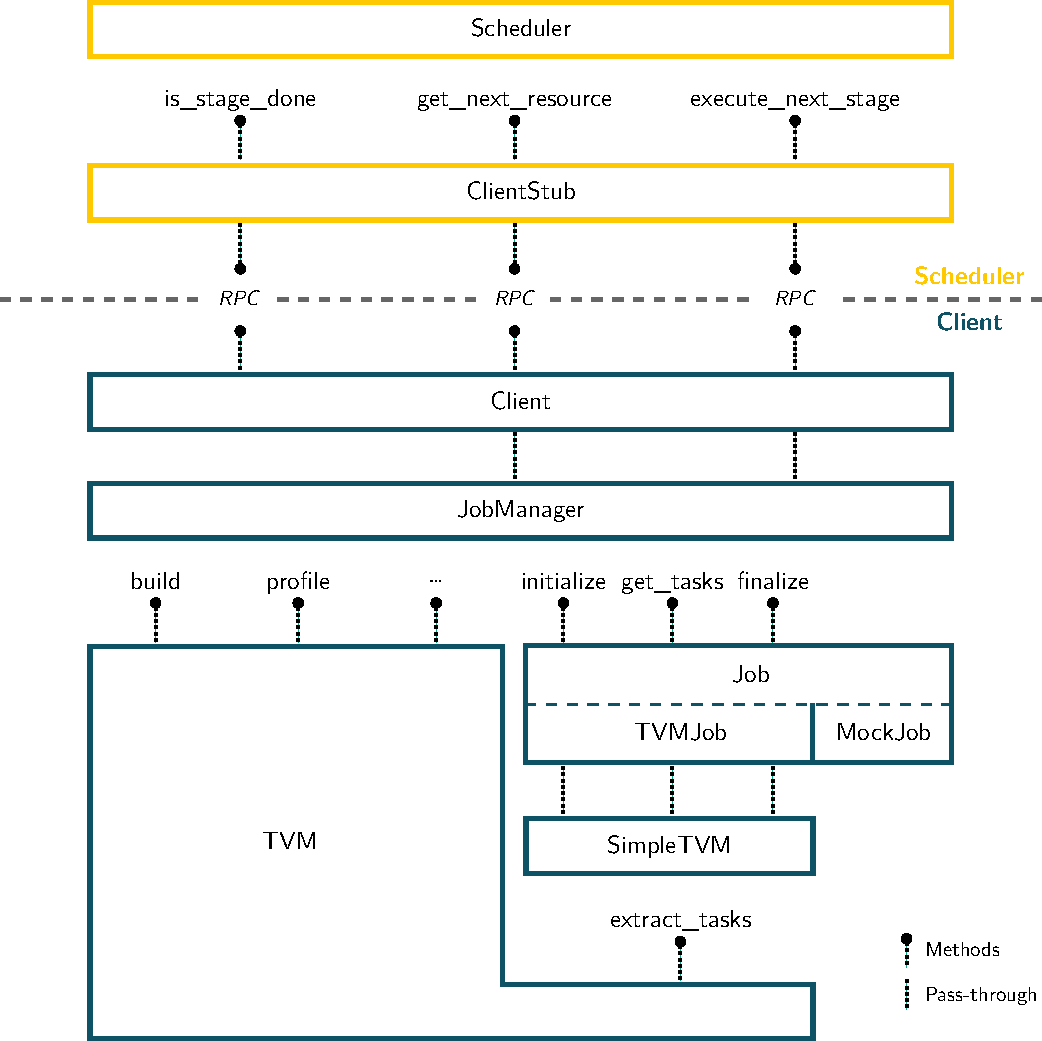
\includegraphics[width=\textwidth]{scheduler_layers}%
	\caption{Layers and components of scheduler implementation}
	\label{fig:scheduler-layers}
\end{figure}

The components act as layers of abstraction sitting on top of TVM to eventually hook into the actual autotuning process. Figure \ref{fig:scheduler-layers} shows the whole stack including method interfaces. We look closer at each component, from top to bottom.
\begin{description}
	\item[Scheduler] The \pythoninline/Scheduler/ implements the interleaved scheduling algorithms from Listings \ref{lst:sched-algo-interleaving-greedy} and  \ref{lst:sched-algo-interleaving-fair} as well as the sequential and synchronous strategies. The strategy can be specified when starting the scheduler. Instead of a list of jobs as in the algorithm, the scheduler actually keeps a list of the clients which run those jobs. The scheduler provides an \gls{rpc} interface for the client to register (not depicted in the figure) and will keep a reference to that client to enable controlling of its autotuning job. Additionally, some error handling is added to, e.g., remove clients if they become unreachable. Resource state is implemented in a resource--to--boolean dictionary, indicating if a given resource is free.
	\item[ClientStub] The \pythoninline/ClientStub/ does not perform any functionality on its own, rather it acts as an abstraction of the \pythoninline/Client/'s \gls{rpc} interface so the scheduler can call client methods as if they were an in-process object, allowing for a clean implementation of the scheduling algorithms. The \pythoninline/ClientStub/ passes through calls to the actual \pythoninline/Client/ but handles \gls{rpc} including serialization/deserialization of variables and error handling.
	\item[Client] The \pythoninline/Client/ provides the interface that is required by the scheduler to control jobs. It registers with the scheduler upon launch and exposes three methods via \gls{rpc}:
	\begin{itemize}
		\item \pythoninline/get_next_resource/ returns the resource that the next stage will run on, or \pythoninline/None/ if the job is complete, effectively combining two functionalities into one method. Furthermore, if the job is complete, the client shuts down after sending the \gls{rpc} response.
		\item \pythoninline/execute_next_stage/ calls the function for the next stage asynchronously and keeps a reference to the stage's thread in form of a future. If another stage is currently running, this methods fails.
		\item \pythoninline/is_stage_done/ returns a boolean, denoting if the stage that was previously executed using \pythoninline/execute_next_stage/ has finished. If no stage has been executed yet or the future indicates that the stage's thread has terminated,  \pythoninline/True/ is returned,  \pythoninline/False/ otherwise.
	\end{itemize}
	\item[JobManager] The \pythoninline/JobManager/ is responsible for negotiating between the simple resource- and stage-based interface required by the scheduler and the more complex interface of TVM's autotuning. This conversion from a stateless to a stateful interface requires that the \pythoninline/JobManager/ keep track of the current progress of the autotuning process, i.e. the position in the autotuning loop identified by task and stage. Effectively, it decides the order of stages in the loop, when the loop starts again, and when the loop terminates. This allows it to implement two methods: \pythoninline/get_next_resource/ is called directly by the client to get the resource that the next stage will run on, \pythoninline/get_next_stage/ returns a method containing the stage functionality which is executed by the client's \pythoninline/execute_next_stage/.\par
	The logic by which the next stage is decided in \pythoninline/get_next_stage/ is presented in Listing \ref{lst:stage-decision-algo}. \pythoninline/get_next_resource/ follows a similar logic but returns the resource instead of methods. The job's state is determined by flags indicating if the job has been initialized and finalized as well as the current task and stage in that task (Lines 1--2). If the job has not been initialized, the initialization method is returned and the \pythoninline/initialized/ flag is set (Lines 4--6). Then, the autotuning loop for the first task is started. With each call of \pythoninline/get_next_stage/, \pythoninline/current_stage/ is incremented and the respective stage's method is returned (Lines 8--22). The stage methods come from either the \pythoninline/Job/ or the decomposed TVM autotuning API. At the end of one loop iteration, which corresponds to one batch, the \pythoninline/current_stage/ is set to the first stage of the loop (Line 21). If the current batch was the last batch of the task (because either the search space has been exhausted or the specified number of trials has been reached), \pythoninline/current_task/ is incremented and \pythoninline/current_stage/ is reset to the task initialization so autotuning can commence for the next task (Lines 15--18). If all tasks have completed, the autotuning job is done (Line 7). Next comes the job finalization method (Lines 23--25), after which \pythoninline/None/ is always returned (Line 26).\par
\begin{listing}[h]
\begin{pythoncode}
initialized = finalized = False
current_task = current_stage = 0

if not initialized:
    initialized = True
    return initialize_job_fn
elif current_task < number_of_tasks:
    current_stage += 1
    if   current_stage == 1: return initialize_task_fn
    elif current_stage == 2: return select_batch_fn
    elif current_stage == 3: return build_fn
    elif current_stage == 4: return profile_fn
    elif current_stage == 5: return update_model_fn
    elif current_stage == 6:
        if last_batch:
            # Go to next task
            current_task += 1
            current_stage = 0
        else:
            # Go to select batch stage
            current_stage = 1
        return finish_batch_fn
elif not finalized:
    finalized = True
    return finalize_job_fn
else: return None
\end{pythoncode}
\unskip
\caption[{Pseudocode of JobManager's stage decision logic}]{Pseudocode of \pythoninline/JobManager/'s stage decision logic}
\label{lst:stage-decision-algo}
\end{listing}
	There is another version called \pythoninline/BundlingJobManager/ which exposes the same interface but instead of returning each stage individually, it bundles the stages for one resource into a single, larger stage. Thus, there are effectively only two stages, one for the client (select configurations, build, update model) and one for the target device (profiling), as opposed to \pythoninline/JobManager/ where each stage is individually schedulable. This might decrease resource idle time and speed up autotuning.
	\item[Job] The \pythoninline/Job/ is an abstract class which acts as interface specification for \pythoninline/TVMJob/ and \pythoninline/MockJob/. Jobs contain a collection of tasks as well as the initialization and finalization methods used by the \pythoninline/JobManager/.
	\item[TVMJob] The \pythoninline/TVMJob/ represents one autotuning job. It only passes calls through to \pythoninline/SimpleTVM/ which contains the implementations. The initialization method only stores a timestamp of the autotuning begin for measurement. The finalization method collects error and time statistics from the autotuning process and inserts them into the benchmarking context. Additionally, it merges the job-specific autotuning database with the global database. The collection of tasks is extracted using a method from TVM, but modified slightly by SimpleTVM.
	\item[MockJob] A \pythoninline/MockJob/ is a drop-in replacement for \pythoninline/TVMJob/, exposing the same interface but not running actual autotuning, which is a slow process. Rather, it simulates work by sleeping and prints to the console when stages are started and finished. This allows rapid debugging of the scheduler algorithms because no infrastructure like servers and the tracker need to be set up. The number of batches and tasks can be specified, as well as a time stretch factor to slow down or speed up the simulated work. The mock stages proportions are about the same as in real autotuning, e.g., profiling takes longer than building. It does not depend on any other components such as TVM.
\end{description}

\subsection{Usage}
Switching from scheduler-less default autotuning to scheduled autotuning is trivial if the former is already being used, as shown in Listing \ref{lst:simpletvm-flow-with-scheduler}. Creation of the \pythoninline/SimpleTVM/ object and import of the model is identical for both variants (Lines 1--2). Default autotuning is started by calling the appropriate method directly with the autotuning options such as number of trials or profiling timeout (Line 5). For scheduled autotuning, a \pythoninline/TVMJob/ needs to be created first (Line 8). A client for the job is then started with the host names of the client and scheduler machines as parameters (Line 9). After autotuning, the optimized module can be built, saved and evaluated as usual (compare Listing \ref{lst:simpletvm-flow}).
\begin{listing}[h]
\begin{pythoncode}
tvm = SimpleTVM(BenchmarkingContext('gpu'), rpc_tracker=('tracker', 9190))
tvm.from_model('resnet')

# Scheduler-less
tvm.autotune(options)

# Scheduled
job = TVMJob(tvm, options)
Client(job, client_host='client', scheduler_host='scheduler').start()
\end{pythoncode}
\unskip
\caption{Comparison of default and scheduled autotuning}
\label{lst:simpletvm-flow-with-scheduler}
\end{listing}

\subsection{Challenges}
For our very first prototype, we wanted all components to run in a single multi-threaded process, so we could evaluate our approach quickly without having to implement the \gls{rpc} protocol. However, Python does not support true multi-threading due to the global interpreter lock. This lock simplifies memory management for the interpreter but only one thread can execute code at a time because of it. Python's recommended replacement is launching other interpreter processes from within the code, however this requires serialization of objects for inter-process communication. Our nested class structures and passing around of methods that are created inside other methods caused problems with this serialization. That is why we had to implement \gls{rpc} before the actual scheduler to enable separate processes from the beginning.

Since multi-job autotuning with a scheduler requires setup of the infrastructure and is rather slow, we created the \pythoninline/MockJob/ class for improved debugging and testing of the scheduler functionality. This allows us to evaluate design choices in the scheduling algorithm much more rapidly. Moreover, the isolation from TVM narrows the room for errors which facilitates focusing on scheduler issues without being disrupted by problems caused by autotuning.

\section{Autotuning as a Service}
Setting up the multi-job autotuning infrastructure is cumbersome because a lot of components need to be configured and deployed, a lot of it imperatively in code. Additionally, provisioning of new client and target machines is not done automatically by the scheduler, which limits the scale at which autotuning can be performed. This motivates the need for an \gls{aaas} platform, which hides the complexity of building and maintaining the infrastructure and thus simplifies the application of autotuning, opening up the opportunities of autotuning for any developer of \gls{dl}-based software.

We imagine a solution that allows users to submit their trained model and a declarative specification, including information such as a target inference time to meet service-level agreements and the target device type such as specialized accelerators. The platform then automatically sets up the required machines and components, runs the autotuning process until the user's target inference time is achieved (or no further optimization is possible), then the optimized version is returned to the user. To this end, we propose a reference architecture. However, we do not implement the platform. \cite{Cho.2019} shows how the Kubernetes container management system could be harnessed for resource provisioning in an \gls{aaas} platform, with a prototype delivering promising results. Our architecture builds on top of such a system, however it does not prescribe any specific product.

\begin{figure}[h]
	\centering
	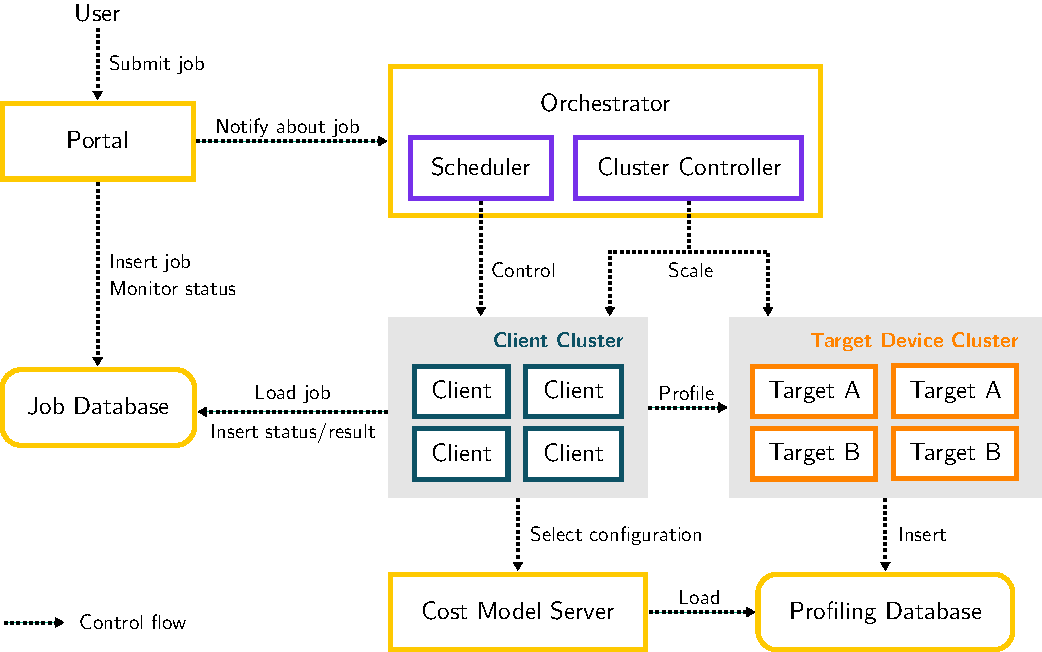
\includegraphics[width=\textwidth]{aaas_architecture}%
	\caption{Autotuning as a Service reference architecture}
	\label{fig:aaas-architecture}
\end{figure}

Figure \ref{fig:aaas-architecture} shows our proposed architecture. Users can submit their jobs including the model and specification through the portal. First the portal inserts that job information in the job database, after which it notifies the orchestrator about the new job. The orchestrator decides if the existing resources are sufficient, or if the client and target device cluster need to be scaled up, e.g., by booting new server instances on a cloud computing platform. The cluster controller, e.g., a Kubernetes Master, is responsible for executing the scaling. Then, the client is created on a client machine and the job is registered with the scheduler.
The scheduler now controls the autotuning jobs as described in the previous sections. However, the actual client functionality changes in the \gls{aaas} scenario. The cost model is extracted to a central server that all clients share, so neither a local cost model nor a job-specific autotuning database is necessary. The cost model server keeps a separate model for every target device. Furthermore, the client does not request profiling servers from a tracker, but the target devices are explicitly assigned per profiling stage by the scheduler. Profiling results are not returned to the client, but inserted into a global profiling database, which the cost model server uses to update the models periodically. Clients store their state in the job database as opposed to the JobManager object, which makes the clients stateless so they can resume the job in case of failure. This also allows the user to monitor autotuning progress through the portal. Once a job has completed, the resulting optimized TVM module is stored in the job database and the user can download it for deployment in his application.

Additionally, we make propose to increase autotuning speed. Firstly, before starting the autotuning, inference performance of a newly submitted model is checked with the existing best configurations. If the user's specifications are already met, no job needs to be launched. Secondly, jobs can be parallelized by splitting them into multiple jobs. Jobs consist of a set of tasks that are independent of each other. Moreover, the search space of each task can be divided to split one task into multiple. Leveraging task-level and search space-level splitting, autotuning can be accelerated if users request a higher number of resource be allocated to them. Furthermore, unused resources can be used better if the total platform load is low.

One limitation of \gls{aaas} over on-premise autotuning infrastructure is the set of supported target devices types. The platform can provide support for common accelerators, but if more exotic or novel hardware is desired, \gls{aaas} will fall short. One solution would be to support profiling on devices outside of the target device cluster. However, appropriate security measures would need to be taken.

In summary, the \gls{aaas} platform makes four important changes to the existing multi-job, scheduled autotuning architecture:
\begin{itemize}
	\item User-friendly portal instead of job specification in code
	\item Automatic resource provisioning/scaling instead of manual infrastructure setup
	\item Shared cost model between clients instead of job-local model
	\item External client state to recover from job failure instead of stateful clients
\end{itemize}
Instantiating such a platform is an important step towards making autotuning more accessible to enable more real-time \gls{dl} applications with little effort for developers.
	\chapter{Evaluation}
	To evaluate the impact of our scheduler, we compare the two approaches from Section \ref{sec:scalability} to our interleaving scheduler which aims to satisfy the \enquote{Optimum} solution. Additionally, we use the sequential scheduling algorithm as baseline while synchronous scheduling represents the worst case by forcing maximum interference. All scenarios are considered in terms of total autotuning completion time, time for the individual stages and the resulting inference performance.

Our evaluation environment consists of two identical machines with the following specifications:
\begin{itemize}
	\item 2x Intel Xeon E5-2650 v3, 10 cores, \SI{2.30}{\giga\hertz}
	\begin{itemize}
		\item Hyper-threading enabled
		\item AVX2 instruction set
	\end{itemize}
	\item \SI{128}{\giga\byte} main memory
	\item 4x Tesla K80 \glspl{gpu}, 4992 CUDA cores, \SI{24}{\giga\byte} memory
	\item Ubuntu 16.04.6 with Linux Kernel 4.4.0
	\item Python 3.6.8
\end{itemize}

Clients always run on the first machine, while profiling servers (TVM RPC servers) always run on the second machine whose \glspl{gpu} are used as target devices. Scheduler and tracker run on the first machine to decrease network latency. They do not interfere with autotuning since they are not computationally intensive.

The number of clients and profiling servers changes for every experiment, as shown in Table \ref{tab:tvm-evaluation-setups}. On \enquote{dedicated} servers, there is only one client. Two clients run on \enquote{shared} servers. Each profiling server of one client is assigned to a different GPU. Without interleaving, each client has its own set of four profiling servers, which might result in two servers if different clients being assigned to the same GPU. However, with interleaving, they can share the servers since they will never profile at the same time, eliminating competition.
\begin{table}
	\newcommand\heading[1]{\textcolor{white}{\textbf{#1}}}
	\renewcommand{\arraystretch}{1.2}
	\sffamily
	\centering
	\begin{tabularx}{\textwidth}{l l l l X}
	\rowcolor{black} \heading{Setup} & \heading{Server~~~~~} & \heading{Scheduler~~~~~~~~~~~~~} & \heading{Bundling~~~} & \heading{Profiling servers} \vspace{2pt} \\
	\textbf{A} & Dedicated & sequential & No & 4 \\
	\textbf{B} & Shared & sequential & No & 8 \\
	\textbf{C} & Shared & synchronous & No & 8 \\
	\textbf{D} & Shared & interleaved-greedy & No & 4 \\
	\textbf{E} & Shared & interleaved-fair & No & 4 \\
	\textbf{F} & Shared & interleaved-greedy & Yes & 4 \\
	\textbf{G} & Shared & interleaved-fair & Yes & 4 \\
	\end{tabularx}
	\caption{Evaluation setups}
	\label{tab:tvm-evaluation-setups}
\end{table}

All setups are controlled by the scheduler so each experiment is affected by the---albeit minimal---overhead of scheduling and \gls{rpc}. Two separate schedulers, one for each client, are used in B to achieve natural interference. \enquote{Bundling} indicates if stages of one resource are bundled into a single stage using the \pythoninline/BundlingJobManager/, or if each stage is individually scheduled.

Our test model is a ResNet-18, which consists of 12 convolution layers and one fully-connected layers, resulting in a job of 13 tasks. We autotune with 2000 trials per task and a profiling timeout of \SI{5}{\second}. Transfer learning from the global autotuning database is disabled so each experiment starts from the same, untrained cost model for a fair comparison. However, transfer learning is enabled between tasks. For time reasons, each experiment is only conducted once so the sample size is small.

A complete chart of all results can be found in Appendix \ref{sec:results}.

\section{Results}
First, we examine the impact of interference that was qualitatively described in Section \ref{sec:scalability}. We compare A, the optimum in terms of autotuning time and inference performance, with B and C (Figure \ref{fig:chart-interference-impact}). B lets jobs naturally interfere, while C forces maximum interference as worst case scenario. Interference is particularly noticeable for model updates since they are rather computationally intensive, which is why we show model update time in every figure.\\
The baseline completion time from A is \SI{14.5}{\hour}, \SI{6.1}{\hour} (42\%) of which are spent updating the model. Natural interference results in an increase in autotuning time by \SI{4.1}{\hour} (+28\%) while forced interference takes even \SI{5.0}{\hour} (+34\%) longer\footnote{For C, the time spent waiting for the other job to finish a stage introduced by the synchronous scheduling algorithm to force interference was subtracted from the total completion time since it would not occur naturally.}. This significant increase can be attributed to slower model updates, which witness a strong decline in performance. Compared with the baseline, the total time spent updating the model increases by \SI{3.8}{\hour} (+62\%) for B and by \SI{5.2}{\hour} (+85\%) for C. Build time only increases marginally, with profiling being slightly faster, possibly due to more timeouts. The baseline inference time is \SI{48.6}{\milli\second}. B is \SI{1.5}{\milli\second} slower, C is \SI{0.5}{\milli\second} slower. 

\begin{figure}[t]
	\begin{minipage}[b]{.6\textwidth}
		\centering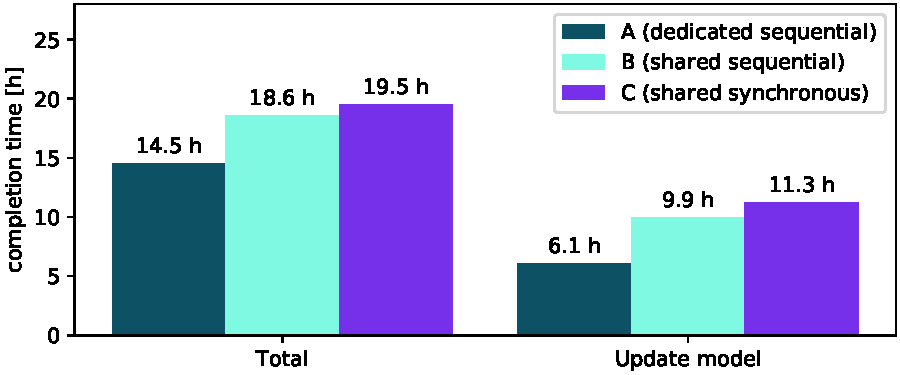
\includegraphics[width=\textwidth]{chart_interference_impact_completion}
		\subcaption{Completion time}\label{fig:chart-interference-impact-completion}
	\end{minipage}%
	\hfill
	\begin{minipage}[b]{.35\textwidth}
		\centering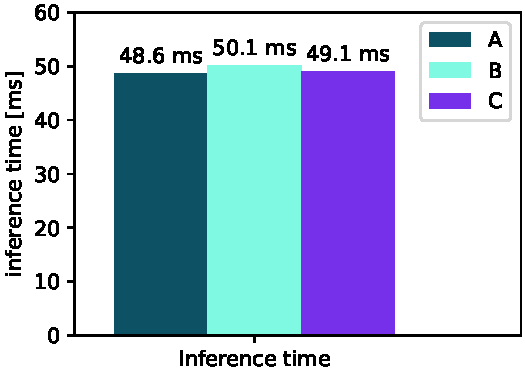
\includegraphics[width=\textwidth]{chart_interference_impact_inference}
		\subcaption{Inference performance}\label{fig:chart-interference-impact-inference}
	\end{minipage}
	\caption{Impact of interference}
	\label{fig:chart-interference-impact}
\end{figure}

We examine experiments D and E to evaluate the greedy and fair scheduler algorithm design, comparing them with A as baseline (Figure \ref{fig:chart-interleaving}). Using greedy interleaving, autotuning completes in \SI{20.4}{\hour}, \SI{5.9}{\hour} slower than A. While model update time stays about the same, \SI{5.5}{\hour} (27\%) of the total time is now spent waiting\footnote{Only stage execution times can be measured. Wait time and non-stage times (transfer learning, file operations) need to be derived. Non-stage times are about \SI{0.49}{\hour}, derived from A. Wait time for interleaving is calculated as follows: $t_{wait} = t_{total} - \sum_{i}t_{stage,i} - \SI{0.49}{\hour}$} for resources to become free to prevent interference. Fair interleaving is impacted even more by waiting, with total autotuning time increasing to \SI{24.1}{\hour}, \SI{9.6}{\hour} (+62\%) slower than A. Model update time remains about the same again, but wait time accumulates to \SI{8.9}{\hour} (37\% of total autotuning). Building and profiling time do not change for both. While the total completion time deteriorates, inference performance matches the baseline of \SI{48.6}{\milli\second} for both D and E.

\begin{figure}[t]
	\begin{minipage}[b]{.6\textwidth}
		\centering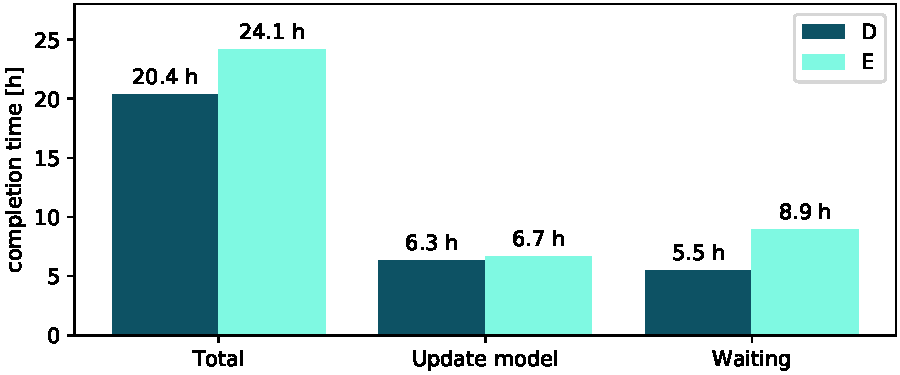
\includegraphics[width=\textwidth]{chart_interleaving_completion}
		\subcaption{Completion time}\label{fig:chart-interleaving-completion}
	\end{minipage}%
	\hfill
	\begin{minipage}[b]{.35\textwidth}
		\centering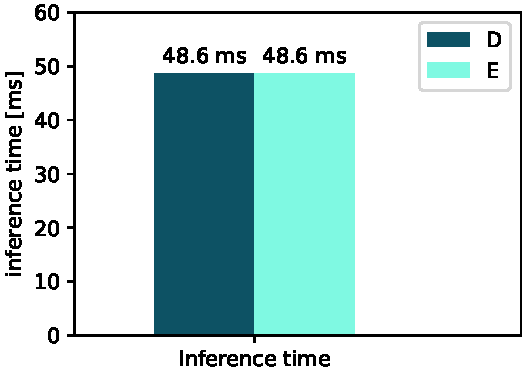
\includegraphics[width=\textwidth]{chart_interleaving_inference}
		\subcaption{Inference performance}\label{fig:chart-interleaving-inference}
	\end{minipage}
	\caption[Results of greedy versus fair interleaving]{Greedy versus fair interleaving}
	\label{fig:chart-interleaving}
\end{figure}

Finally, we examine the effect of employing stage bundling as opposed to individually scheduling them (Figure \ref{fig:chart-bundling}). The greedy algorithm is used in F, the fair algorithm is used in G. With bundling, greedy interleaving performs about the same as without bundling. On the other hand, fair interleaving completes \SI{2.4}{\hour} (-10\%) earlier than the individually scheduled version due to a total wait time that is \SI{2.7}{\hour} (-30\%) shorter. As before, model update time remains relatively similar. Inference time in F is \SI{0.4}{\milli\second} faster than in D, while G's is slower than E by \SI{0.3}{\milli\second}.

\begin{figure}[t]
	\begin{minipage}[b]{.6\textwidth}
		\centering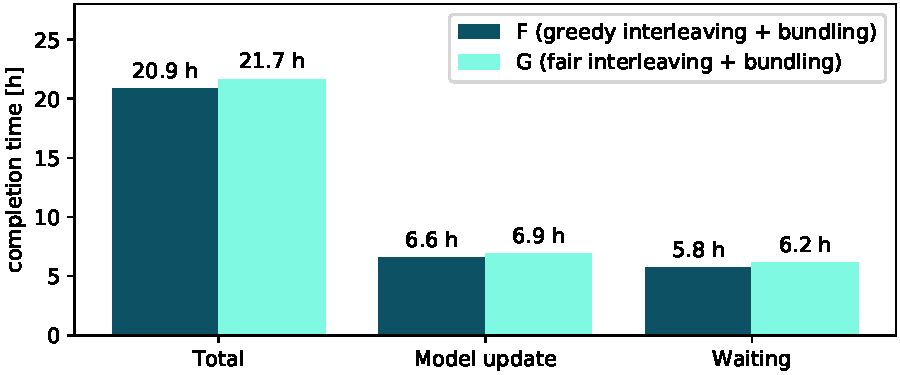
\includegraphics[width=\textwidth]{chart_bundling_completion}
		\subcaption{Completion time}\label{fig:chart-bundling-completion}
	\end{minipage}%
	\hfill
	\begin{minipage}[b]{.35\textwidth}
		\centering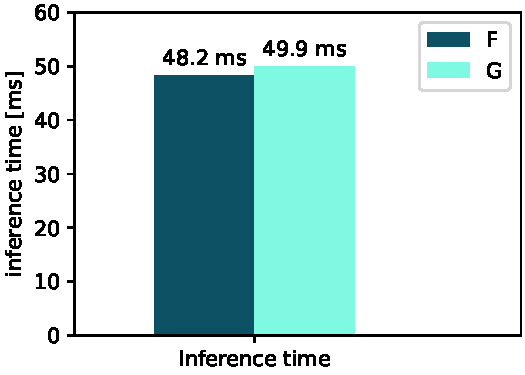
\includegraphics[width=\textwidth]{chart_bundling_inference}
		\subcaption{Inference performance}\label{fig:chart-bundling-inference}
	\end{minipage}
	\caption[Results of greedy versus fair interleaving with bundling]{Greedy versus fair interleaving with bundling}
	\label{fig:chart-bundling}
\end{figure}

\section{Discussion}
The objective of large-scale autotuning is to achieve the autotuning time and inference performance of running only a single job on each server, but with shared resources to keep the amount of required hardware at a minimum. Single-job autotuning is represented by Setup A, which is why we use it as baseline for comparisons with the other experiments. Because our evaluation is limited to a single machine type and model, more experiments are required for a general analysis.

In B and C we show the detrimental effects of interference on performance which motivated the creation of a scheduler. If it were not for this, resources could be shared and jobs could be run in parallel without control by a central entity. B and C behave relatively similar because even without explicit scheduling, both jobs run approximately synchronous since they autotune the same model. In real-world scenarios with diverse workloads, there might be a more drastic difference between B and C. The fact that C has faster inference than B is presumably caused by the probabilistic nature of configuration selection. The difference in inference performance of both to the baseline is relatively small due to the large number of trials which even out the impact of interference. However, even slightly worse inference speed has a large impact with an increasing number of inferences.

Note how interference is avoided with the scheduler in D--G, which manifests in stage times (particularly model updating) that are comparable to single-job autotuning as well as in a good inference performance. However, a significant amount of wait time is introduced which drives up total completion time. Greedy interleaving without bundling shows the shortest wait time in our experiments. Bundling does not show a big effect when comparing D and F because greedy interleaving naturally behaves like bundling. However, fair interleaving benefits much from bundling in our experiments, remedying the vast wait time.

Greedy interleaving works well in our experiments because both jobs are identical and the portion of time spent on the client machine versus time spent on the target device is roughly similar. As a result, wait time is reduced because, after an initial wait period, both jobs alternate nearly perfectly but mutually opposing between client and target. Despite these results, we believe that fair interleaving is the superior algorithm for scheduling heterogeneous jobs with varying complexity on a large scale, as would be the case with \gls{aaas}. Greedy interleaving would allow jobs to monopolize resources for an extended period of time, while fair interleaving allows for a finer control, especially if more resources are available. Bundling in conjunction with the fair algorithm is still an option to interleave homogeneous jobs on few resources, which would show the same effect as the greedy algorithm in our experiment.

Our scheduler is very rudimentary at this point, leaving much room for improvement. While the concept of interleaving seems promising, a more intelligent approach than fair round-robin could be employed to fill idle time optimally while keeping average wait time low. For example, a predictive scheduler could use knowledge from previous tasks to make a more educated decision that will maximize resource utilization. This would augment the notion of load-awareness with knowledge about the estimated stage execution time. Such a scheduler could then leverage the exact or heuristic interleaving algorithm from \cite{Ma.2005}. However, a more sophisticated algorithm might require finer control over the stages, which cannot be provided by the client's current resource/stage interface. Trading off a complex client but simple scheduler for a thin, stateless client and autotuning-aware scheduler by shifting responsibilities might become a necessity.

Furthermore, the scheduler needs to be enhanced with support for multiple resources of the same type. At this point, all target devices are regarded as a single, atomic resource. More granularity is essential for production-grade implementations in an \gls{aaas} platform. This would go hand in hand with eliminating the tracker and letting the scheduler assign target devices to clients. A trivial refinement is replacing the busy waiting for a stage to be done in the scheduler algorithm, resulting in an excess of redundant \gls{rpc} calls, by a push-based approach, where the client notifies the scheduler once a stage has completed.

We used our scheduler only for autotuning with TVM. However, other autotuning frameworks like \gls{tc} that have the same scaling issues might also profit from our solution. The \gls{aaas} platform might even provide support for a variety of autotuning frameworks.
	\chapter{Conclusion}
	Enabling large-scale autotuning is the foundation of any \gls{aaas} platform that uses our reference architecture. We demonstrated that our interleaving scheduler can leverage the fundamental weakness of resource idle time to make sharing of computation resources possible, which facilitates fast and economical autotuning while delivering good inference performance. This is a key step towards democratizing real-time \gls{dl} applications to power exciting innovations in a wide variety of fields.

Future efforts based on our work should focus on creating a more intelligent scheduler algorithm to improve the efficiency of multi-job autotuning. A resource provisioning algorithm will then complete the orchestrator component, paving the way for the development of a mature \gls{aaas} product.

	
	\clearpage
	
	%----------------------------------------------------------------------------
	% Appendix
	%----------------------------------------------------------------------------
	
	\cleardoublepage
	\printbibliography

	\printglossary[style=altlist]
	
	\clearpage
	\appendix
\end{document}